\documentclass[11pt]{article}
\usepackage[preprint]{acl}
\usepackage{times}
\usepackage{latexsym}
\usepackage[T1]{fontenc}
\usepackage[utf8]{inputenc}
\usepackage{microtype}
\usepackage{inconsolata}
\usepackage{graphicx}
\usepackage{booktabs}
\usepackage{amsmath}
\usepackage{xspace}

% Result numbers are generated by `active-gliner analyse` into numbers.tex.
% Never type a result by hand (AGENTS.md rule 10). Missing numbers show as ??.
\InputIfFileExists{numbers.tex}{}{}
\newcommand{\res}[1]{\ifcsname #1\endcsname\csname #1\endcsname\else\textbf{??}\fi}

\title{Active GLiNER: Which Examples Should LLMs Label?}

\author{Abhishek Thomas \\
  Independent researcher, Paris, France \\
  \texttt{abhi@recolli.com}}

\begin{document}
\maketitle

\begin{abstract}
Small extraction models such as GLiNER can be trained on labels produced by a large language model (LLM), which makes annotation cheap but noisy. We ask a simple question: when the LLM can label only a few hundred examples, should the small model choose which ones? We study one round of uncertainty-based selection with a GLiNER2.5 student and LLM teachers on four extraction tasks and six datasets: named entity recognition (CleanCoNLL, BC5CDR, MIT Movie), relation prediction (CrossRE), multi-label classification (Hallmarks of Cancer) and slot extraction to JSON (MASSIVE, English and French). Our pre-registered primary contrast is the interaction between selection and label source: whether choosing the student's least confident examples helps less when an LLM, rather than ground truth, provides the labels. The answer depends on the task. For NER, min selection loses to random under both label sources (min minus random is \res{PracticalNER} F1 points with LLM labels), mostly because it picks sentences where the student predicts nothing; ranking those last reverses the loss on CleanCoNLL. For relations, min helps with ground truth, and LLM label errors remove most of that gain. LLM errors concentrate where the student is unsure only for NER. For NER, a student trained on 400 LLM-labelled sentences comes close to its teacher (\res{DeployStudentGemmaRandom} against \res{DeployTeacher} F1) at \res{DeploySpeedup} times the speed, and on some datasets students beat their teacher. Replicating an earlier thesis on all datasets, we find that its three uncertainty scores (mean confidence, MSE, MNLP) select identical sentences, because every pool holds more empty-prediction sentences than the budget, and that half ground truth matches full ground truth only on MIT Movie.
We release the code as a command-line tool, together with all teacher labels, adapters and run logs.
\end{abstract}

\section{Introduction}

Information extraction models that run on a CPU in milliseconds are attractive for production, but they need labelled data for every new domain. Large language models can now produce those labels \citep{llmaaa2023,llmsloop2024}, and a small student trained on LLM labels can match or beat its teacher at a fraction of the cost \citep{clinicalie2025}. GLiNER \citep{gliner2023} and GLiNER2 \citep{gliner2_2025} made such students general: one encoder handles entities, relations, classification and structured output from a schema.

If an LLM labels the data, the next question is which data it should label. Active learning answers this for human annotators: pick the examples the current model is least sure about. Yet active learning often fails to beat random selection \citep{fragility2024,chemal2026,partingillusions2019}, and LLM labels change the picture. The examples a student finds hardest may also be the examples an LLM gets wrong, so uncertainty could select exactly the noisiest labels. \citet{humansloop2026} even find that labelling the whole pool with an LLM beats active learning.

We test this directly. Our question is: \emph{when does student uncertainty improve one-round LLM annotation, and when does teacher error erase that benefit?} We make four contributions.

\begin{enumerate}
\item A pre-registered comparison of uncertainty and random selection, crossed with ground truth and LLM labels, on four tasks and six datasets, with five seeds on primary cells, paired bootstrap intervals and Holm correction.
\item An analysis of teacher errors by student confidence: do LLM mistakes concentrate where the student is unsure (Q2), do different LLMs fail on the same examples (Q3), and do larger teachers label better (Q4)?
\item Cost, latency and size views of students and teachers, including a Pareto front and a quality-latency quadrant chart.
\item An open command-line tool that runs the whole loop (score, select, label with any OpenAI-compatible endpoint, train with LoRA, report), with every paper run reproducible through it.
\end{enumerate}

This paper builds on the author's master thesis, which studied the same loop for NER on MIT Movie with GLiNER and Gemma~3. Section~\ref{sec:thesis} lists what the thesis did, what it found, and which of its protocol problems this study fixes.

\section{Related work}

\paragraph{Active learning with LLM annotators.} LLMaAA \citep{llmaaa2023} uses an LLM as the annotator inside active learning for NER and relation extraction. \citet{llmsloop2024} report that GPT-4 labels in the loop are 42 times cheaper for low-resource NER. ALLabel \citep{allabel2025} selects demonstrations for the LLM rather than training data for a student. \citet{mixllm2026} combine several small LLMs and use their disagreement to flag errors, and HyPAC \citep{hypac2026} routes examples between fast and slow LLMs and humans with an error guarantee. Active knowledge distillation \citep{activekd2025} sends uncertain examples to an LLM teacher for classification. We differ in the student (a schema-driven GLiNER2.5 model), the breadth of tasks, and the explicit test of whether teacher error cancels the gain from selection.

\paragraph{Doubts about active learning.} Random selection is a strong baseline \citep{fragility2024,partingillusions2019}. For NER, \citet{chemal2026} find uncertainty and diversity rules unstable, and a scoping review finds that only 13 of 62 studies report run time \citep{alnerreview2024}. Practitioners cite setup effort and unclear savings as blockers \citep{reassessal2026}. We therefore pre-register the contrast, report seeds and intervals, and release a tool.

\paragraph{LLM-to-small-model distillation.} GLiNER-BioMed \citep{glinerbiomed2025} and FiNERweb \citep{finerweb2025} train GLiNER-style students on LLM labels without selection. \citet{clinicalie2025} show that a distilled BERT can beat its teacher. \citet{noisyner2026} reweight noisy LLM NER labels by error type.

\paragraph{GLiNER and pre-annotation.} The closest work to ours outside arXiv uses zero-shot GLiNER to pre-annotate hiking descriptions for human correction and retrains over three rounds \citep{tafer2026hiking}; it has no selection rule and no random comparison.

\paragraph{Uncertainty in extraction.} Span probabilities can stay informative under domain shift \citep{finner2026}; calibration metrics for NER are discussed by \citet{nercalib2024}. Classic active learning for NER uses sequence-level uncertainty such as MNLP \citep{mnlp2017}.

\section{Setup}
\label{sec:setup}

\subsection{Tasks and data}

Table~\ref{tab:data} lists the six datasets. We chose sets that are small (at most about 15k training sentences), carefully annotated, and cover four output structures.

\begin{table*}[t]
\centering
\small
\resizebox{\textwidth}{!}{%
\begin{tabular}{llrrrl}
\toprule
Task & Dataset & Pool & Dev & Test & Labels \\
\midrule
NER & CleanCoNLL \citep{cleanconll2023,tjongkimsang2003conll} & 13{,}957 & 3{,}233 & 3{,}427 & 4 types \\
NER & BC5CDR \citep{li2016bc5cdr} & 5{,}228 & 5{,}330 & 5{,}865 & chemical, disease \\
NER & MIT Movie, corrected \citep{liu2013mitmovie,galileo2022mitmovie} & 8{,}797 & 978 & 2{,}443 & 12 types \\
Relations & CrossRE, 6 domains \citep{crossre2022} & 2{,}519 & 300 & 2{,}446 & 17 relation types \\
Multi-label & Hallmarks of Cancer \citep{baker2016hallmarks} & 12{,}119 & 1{,}798 & 3{,}547 & 10 hallmarks \\
Slots (JSON) & MASSIVE 1.1 en-US and fr-FR \citep{massive2022} & 11{,}514 & 2{,}033 & 2{,}974 & 55 slot types \\
\bottomrule
\end{tabular}}
\caption{Datasets. MIT Movie has no official dev split: we hold out a seeded 10\% of train. CrossRE pools train and dev and holds out 300 sentences as dev. Documents never cross splits in BC5CDR, CleanCoNLL and Hallmarks. Sentences with no gold label stay in the pool.}
\label{tab:data}
\end{table*}

For CrossRE we use an adapted protocol: entity mentions are given as input to every model, and the task is to predict all relation types for every ordered pair of mentions, including pairs with no relation. End-to-end triple extraction was too hard for both students and teachers to support a comparison (pilot micro-F1 below 0.08).

\subsection{Student}

The student is GLiNER2.5-multi \citep{gliner25multi} (287M parameters, mDeBERTa-v3-base encoder), loaded from a pinned snapshot, trained with LoRA \citep{lora2021} through the \texttt{gliner2} trainer. Every run starts from a fresh copy of the base model. Hyperparameters come from one Optuna search per task on the dev set (20 trials, the first being the vendor-recommended recipe), frozen before any main run. Training stops after three dev checks without improvement, and the checkpoint with the best dev micro-F1 is kept. CrossRE is the exception: its dev score moves up and down between checks, so every CrossRE run trains all 1000 steps and keeps its best dev checkpoint. For CrossRE the student scores each ordered mention pair with the checkpoint's pretrained relation scorer, applied to the given mention offsets, so that its zero-shot confidence is meaningful for selection. All runs use deterministic GPU kernels in full fp32 precision without TF32, so a seed fixes the result.

\subsection{Teachers}

The main teacher is Gemma~4 12B (QAT, 4-bit GGUF) served locally with llama.cpp at temperature 0 with JSON-schema constrained output. One prompt per task gives the label names and, where a dev check showed it helped, one short definition per label from the annotation guidelines. The same prompt is used for every teacher. Teacher answers are validated: labels must be allowed and spans must occur exactly in the text, starting and ending on a word boundary of the student's tokeniser. A mention that occurs only inside a longer word (for example the rating ``r'' inside ``rated'') is dropped and counted as a teacher error. Teacher labels are cached, so every arm and seed sees the same labels for the same sentence.

\subsection{Selection}

From a frozen pool, a selector picks $N$ sentences in one round. \textbf{Random} samples uniformly. \textbf{Min} scores every sentence with the zero-shot student and picks the lowest sentence confidence: the minimum span confidence for NER (no prediction counts as 0), the minimum distance of any label probability to the threshold for classification and relations, and for slots the minimum value confidence or, if nothing is predicted, one minus the highest below-threshold candidate. \textbf{Diversity} (NER only) clusters student sentence embeddings with $k$-means and takes the sentence nearest each centroid. Pool scores and embeddings are computed once and shared, so paired arms select identical sentences. Because ``no prediction counts as 0'' makes min prefer sentences where the student predicts nothing, a pre-registered sensitivity block on CleanCoNLL ranks such sentences last instead.

\subsection{Protocol and statistics}

Budgets are $N \in \{100, 400\}$ sentences (CrossRE $\{100, 200\}$). Primary cells (min and random, ground truth and Gemma, at the larger budget) have five seeds, all other cells three. Each seed sets pool tie-breaks, data order and LoRA initialisation. We report strict micro-F1 on the official test set; the test set is used once, for final scores only. Two references bound every cell: a lower bound from four zero-shot GLiNER2 models (small, base and multi from GLiNER2.5, and GLiNER2 large), each with its threshold chosen on dev, and an upper bound from training the student on the whole pool, once with ground truth and once with Gemma labels.

The pre-registered primary contrast, per task, is the interaction
\begin{align*}
\Delta = {} & (\text{min} - \text{random})_{\text{Gemma}} \\
& - (\text{min} - \text{random})_{\text{ground truth}},
\end{align*}
paired by seed and, for NER, pooled with equal weight over the three datasets. The four interactions form one Holm family; the four practical contrasts $(\text{min} - \text{random})_{\text{Gemma}}$ form a second. We report seed spread, paired test-set bootstrap intervals \citep{dror2018hitchhiker} and ASO \citep{dror2019deepdominance,ulmer2022deepsig}.

\section{Results}
\label{sec:results}

All numbers below come from \res{FinishedRuns} finished runs through \texttt{active-gliner analyse}. Intervals are 95\% paired bootstrap intervals over test sentences; they do not include seed variation, so we give the seed standard deviation (SD) of each contrast as well.

\begin{table*}[t]
\centering
\small
\resizebox{\textwidth}{!}{\InputIfFileExists{tables/main_results.tex}{}{\textbf{??}}}
\caption{Test micro-F1 (\%) at the main budget ($N = 400$; CrossRE $N = 200$): mean $\pm$ seed SD (number of seeds). Zero-shot is the untrained student with a dev-chosen threshold. Whole pool is one seed. Generated by \texttt{active-gliner analyse}.}
\label{tab:main}
\end{table*}

\begin{figure}[t]
\centering
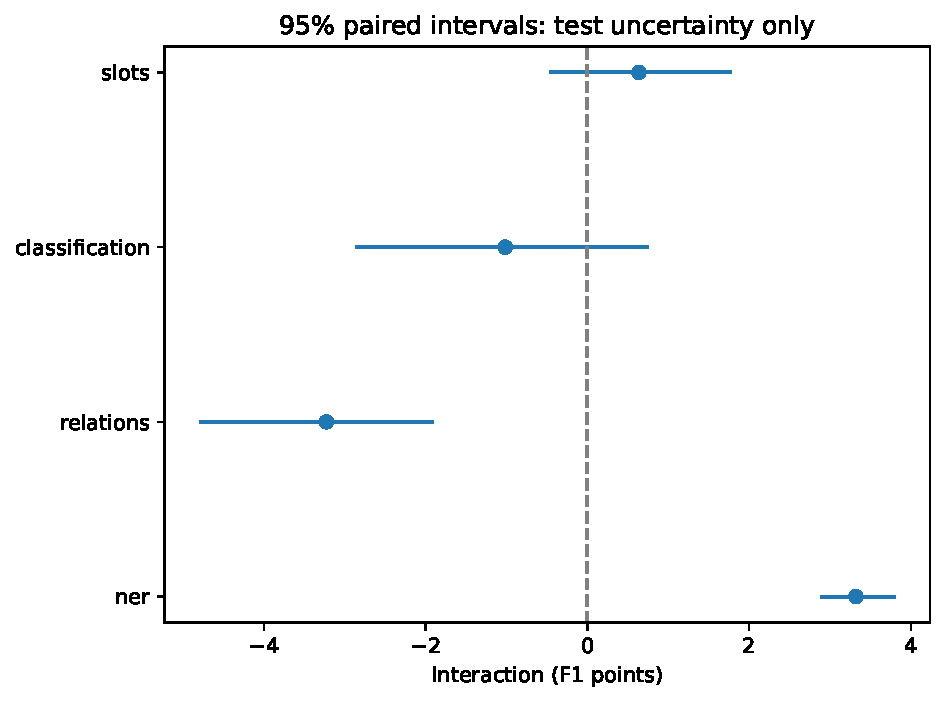
\includegraphics[width=\columnwidth]{figures/interaction-forest.pdf}
\caption{Primary interaction $\Delta$ per task with 95\% paired bootstrap intervals (test uncertainty only). Positive: min loses less against random with Gemma labels than with ground truth.}
\label{fig:interaction}
\end{figure}

\paragraph{Q1: does uncertainty selection help, with ground truth and with LLM labels?} Table~\ref{tab:main} gives every cell and Figure~\ref{fig:interaction} the primary contrast. The interaction $\Delta$ is \res{PrimaryNER} F1 points for NER (95\% interval \res{PrimaryNERLow} to \res{PrimaryNERHigh}, Holm-adjusted $p$\,\res{PrimaryNERP}, seed SD \res{PrimaryNERSd}), \res{PrimaryRelations} for relations (\res{PrimaryRelationsLow} to \res{PrimaryRelationsHigh}, $p$\,\res{PrimaryRelationsP}, SD \res{PrimaryRelationsSd}), \res{PrimaryClassification} for classification (\res{PrimaryClassificationLow} to \res{PrimaryClassificationHigh}, $p$\,\res{PrimaryClassificationP}) and \res{PrimarySlots} for slots (\res{PrimarySlotsLow} to \res{PrimarySlotsHigh}, $p$\,\res{PrimarySlotsP}). The practical contrast, min minus random with Gemma labels, is \res{PracticalNER} for NER (\res{PracticalNERLow} to \res{PracticalNERHigh}, $p$\,\res{PracticalNERP}), \res{PracticalRelations} for relations (\res{PracticalRelationsLow} to \res{PracticalRelationsHigh}, $p$\,\res{PracticalRelationsP}), \res{PracticalClassification} for classification (\res{PracticalClassificationLow} to \res{PracticalClassificationHigh}, $p$\,\res{PracticalClassificationP}) and \res{PracticalSlots} for slots (\res{PracticalSlotsLow} to \res{PracticalSlotsHigh}, $p$\,\res{PracticalSlotsP}).

The two contrasts must be read together. For NER, the interaction is positive because min loses to random under both label sources and loses less with Gemma labels; there is no gain for teacher error to erase. For relations, the pre-registered pattern appears: with ground truth, min beats random (\res{CrossREGroundTruthMin} against \res{CrossREGroundTruthRandom}), and with Gemma labels most of that gain is gone (\res{CrossREGemmaMin} against \res{CrossREGemmaRandom}). For classification, min loses under both sources. For slots, the selectors differ little, and the practical interval includes zero. The NER interaction varies across datasets: its seed SD is close to its mean, and on BC5CDR min loses about as much under both label sources, so the interaction there is near zero (Table~\ref{tab:main}).

On CleanCoNLL, the no-prediction sensitivity block separates two effects. With ground truth, min scores \res{CleanCoNLLGroundTruthMin}, min with empty sentences ranked last \res{CleanCoNLLGroundTruthMinLast}, and random \res{CleanCoNLLGroundTruthRandom}. With Gemma labels the same three arms score \res{CleanCoNLLGemmaMin}, \res{CleanCoNLLGemmaMinLast} and \res{CleanCoNLLGemmaRandom}, and training on the whole Gemma-labelled pool scores \res{CleanCoNLLGemmaWholePool}. Most of the loss of min therefore comes from the rule that sentences with no prediction count as least confident: min then spends the budget on sentences where the student predicts nothing. With that rule reversed and Gemma labels, 400 selected sentences match or exceed the whole labelled pool on this dataset. This is one dataset and a sensitivity analysis, not a pre-registered contrast.

\begin{figure}[t]
\centering
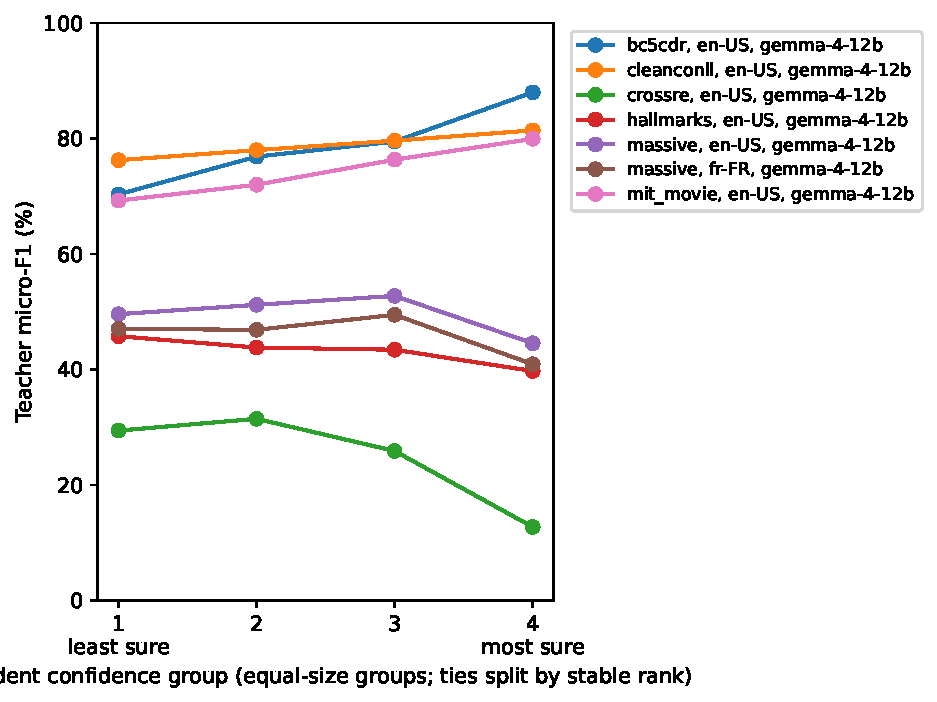
\includegraphics[width=\columnwidth]{figures/teacher-bins.pdf}
\caption{Gemma~4 12B micro-F1 on the pool, by the zero-shot student's sentence confidence (four equal-size groups).}
\label{fig:bins}
\end{figure}

\paragraph{Q2: are LLM errors where the student is unsure?} For NER, yes (Figure~\ref{fig:bins}). Gemma's F1 rises from the student's least sure quarter to its most sure quarter: \res{TeacherBCfiveCDRLeastSure} to \res{TeacherBCfiveCDRMostSure} on BC5CDR, \res{TeacherMITMovieLeastSure} to \res{TeacherMITMovieMostSure} on MIT Movie and \res{TeacherCleanCoNLLLeastSure} to \res{TeacherCleanCoNLLMostSure} on CleanCoNLL. So uncertainty selection sends the teacher the sentences it labels worst. For the other tasks the pattern reverses at the top: the teacher is weakest where the student is most sure (CrossRE \res{TeacherCrossRELeastSure} against \res{TeacherCrossREMostSure}, Hallmarks \res{TeacherHallmarksLeastSure} against \res{TeacherHallmarksMostSure}, MASSIVE English \res{TeacherMassiveEnLeastSure} against \res{TeacherMassiveEnMostSure}). The bins alone do not predict the sign of the interaction: NER, where teacher errors follow student doubt, has a positive $\Delta$, and relations, where they do not, has a negative one. The level of teacher error matters more: Gemma reaches only \res{TeacherCrossRE} F1 on CrossRE test, so any selected set carries many wrong labels.

\paragraph{Q3 and Q4: do teachers fail on the same examples, and do larger teachers label better?} We compare Gemma~4 12B with the smaller Gemma~4 E4B on frozen, stratified test samples (up to 1{,}000 sentences, whole documents where the corpus has them), weighting each sentence by its inclusion probability. The larger teacher is better on five of six English datasets: by \res{LadderBCfiveCDRGap} points on BC5CDR (\res{LadderBCfiveCDRGapLow} to \res{LadderBCfiveCDRGapHigh}), \res{LadderCleanCoNLLGap} on CleanCoNLL (\res{LadderCleanCoNLLGapLow} to \res{LadderCleanCoNLLGapHigh}), \res{LadderMITMovieGap} on MIT Movie (\res{LadderMITMovieGapLow} to \res{LadderMITMovieGapHigh}), \res{LadderHallmarksGap} on Hallmarks (\res{LadderHallmarksGapLow} to \res{LadderHallmarksGapHigh}) and \res{LadderMassiveEnGap} on MASSIVE (\res{LadderMassiveEnGapLow} to \res{LadderMassiveEnGapHigh}). On CrossRE both fail alike (\res{LadderCrossRETwelveB} against \res{LadderCrossREEfourB}; gap interval \res{LadderCrossREGapLow} to \res{LadderCrossREGapHigh}). The two teachers err on largely the same sentences: the Jaccard overlap of their error sentences is between \res{LadderMITMovieOverlap} (MIT Movie) and \res{LadderCleanCoNLLOverlap} (CleanCoNLL), and \res{LadderCrossREOverlap} on CrossRE. Both teachers come from one model family; the planned teachers from other families were not run (Limitations), so we cannot say whether errors are shared across families. The CleanCoNLL sample holds few documents, so its level estimate (\res{LadderCleanCoNLLTwelveB} for 12B) differs from the full test score (\res{TeacherCleanCoNLL}); the paired gap uses the same sentences for both teachers and is not affected by this.

\paragraph{Q5 and Q6: better teachers, better students? Can the student beat its teacher?} A better teacher gives a better student where we can test it: with 400 random sentences, E4B labels train a student to \res{CleanCoNLLEfourBRandom} on CleanCoNLL and \res{HallmarksEfourBRandom} on Hallmarks, against \res{CleanCoNLLGemmaRandom} and \res{HallmarksGemmaRandom} with 12B labels (three seeds each). The student can beat its teacher. Trained on the whole Gemma-labelled pool (one seed), it exceeds Gemma's own test F1 on MIT Movie (\res{MITMovieGemmaWholePool} against \res{TeacherMITMovie}), BC5CDR (\res{BCfiveCDRGemmaWholePool} against \res{TeacherBCfiveCDR}) and MASSIVE English (\res{MassiveEnGemmaWholePool} against \res{TeacherMassiveEn}); with only 400 random sentences it already does so on MIT Movie (\res{MITMovieGemmaRandom}) and MASSIVE French (\res{MassiveFrGemmaRandom} against \res{TeacherMassiveFr}). On CrossRE it stays far below the teacher (\res{CrossREGemmaWholePool} against \res{TeacherCrossRE}), and the whole-pool CrossRE student trained on Gemma labels scores lower than the one trained on 200 random sentences.

\paragraph{Mixing ground truth into LLM labels.} The thesis found on MIT Movie that a share of ground truth closes most of the gap to a fully human-labelled set. We repeat this on every dataset with min selection at the main budget: a random fraction of the selected sentences gets ground truth and the rest keeps Gemma labels (three seeds per cell; Table~\ref{tab:mixing}). MIT Movie reproduces the thesis: 50\% ground truth (\res{MITMovieMixFifty}) already matches all ground truth (\res{MITMovieGroundTruthMin}). No other dataset does. On CrossRE and MASSIVE every extra share helps by a similar step (CrossRE \res{CrossREGemmaMin}, \res{CrossREMixTwentyFive}, \res{CrossREMixFifty}, \res{CrossREMixSeventyFive}, \res{CrossREGroundTruthMin}), and on CleanCoNLL, BC5CDR and Hallmarks the first 25\% gives almost nothing. So a small human share is not a general substitute for full human labelling. A natural idea is to send the human labels to the sentences the student is least sure about. At 25\% this does not help: routed ground truth scores \res{BCfiveCDRMixTwentyFiveRouted} against \res{BCfiveCDRMixTwentyFive} for a random share on BC5CDR, \res{CleanCoNLLMixTwentyFiveRouted} against \res{CleanCoNLLMixTwentyFive} on CleanCoNLL, and \res{MITMovieMixTwentyFiveRouted} against \res{MITMovieMixTwentyFive} on MIT Movie.

\begin{table}[t]
\centering
\footnotesize
\setlength{\tabcolsep}{2.8pt}
\begin{tabular}{lrrrrrr}
\toprule
 & \multicolumn{5}{c}{Ground-truth share} & Routed \\
Dataset & 0\% & 25\% & 50\% & 75\% & 100\% & 25\% \\
\midrule
CleanCoNLL & \res{CleanCoNLLGemmaMin} & \res{CleanCoNLLMixTwentyFive} & \res{CleanCoNLLMixFifty} & \res{CleanCoNLLMixSeventyFive} & \res{CleanCoNLLGroundTruthMin} & \res{CleanCoNLLMixTwentyFiveRouted} \\
BC5CDR & \res{BCfiveCDRGemmaMin} & \res{BCfiveCDRMixTwentyFive} & \res{BCfiveCDRMixFifty} & \res{BCfiveCDRMixSeventyFive} & \res{BCfiveCDRGroundTruthMin} & \res{BCfiveCDRMixTwentyFiveRouted} \\
MIT Movie & \res{MITMovieGemmaMin} & \res{MITMovieMixTwentyFive} & \res{MITMovieMixFifty} & \res{MITMovieMixSeventyFive} & \res{MITMovieGroundTruthMin} & \res{MITMovieMixTwentyFiveRouted} \\
CrossRE & \res{CrossREGemmaMin} & \res{CrossREMixTwentyFive} & \res{CrossREMixFifty} & \res{CrossREMixSeventyFive} & \res{CrossREGroundTruthMin} & -- \\
Hallmarks & \res{HallmarksGemmaMin} & \res{HallmarksMixTwentyFive} & \res{HallmarksMixFifty} & \res{HallmarksMixSeventyFive} & \res{HallmarksGroundTruthMin} & -- \\
MASSIVE en & \res{MassiveEnGemmaMin} & \res{MassiveEnMixTwentyFive} & \res{MassiveEnMixFifty} & \res{MassiveEnMixSeventyFive} & \res{MassiveEnGroundTruthMin} & -- \\
MASSIVE fr & \res{MassiveFrGemmaMin} & \res{MassiveFrMixTwentyFive} & \res{MassiveFrMixFifty} & \res{MassiveFrMixSeventyFive} & \res{MassiveFrGroundTruthMin} & -- \\
\bottomrule
\end{tabular}
\caption{Mixing: test micro-F1 (\%) with min selection at the main budget, mean of three seeds (0\% and 100\%: five seeds; MASSIVE fr: three). The rest of each set keeps Gemma~4 12B labels. Routed: the ground-truth share goes to the least confident sentences.}
\label{tab:mixing}
\end{table}

\begin{figure}[t]
\centering
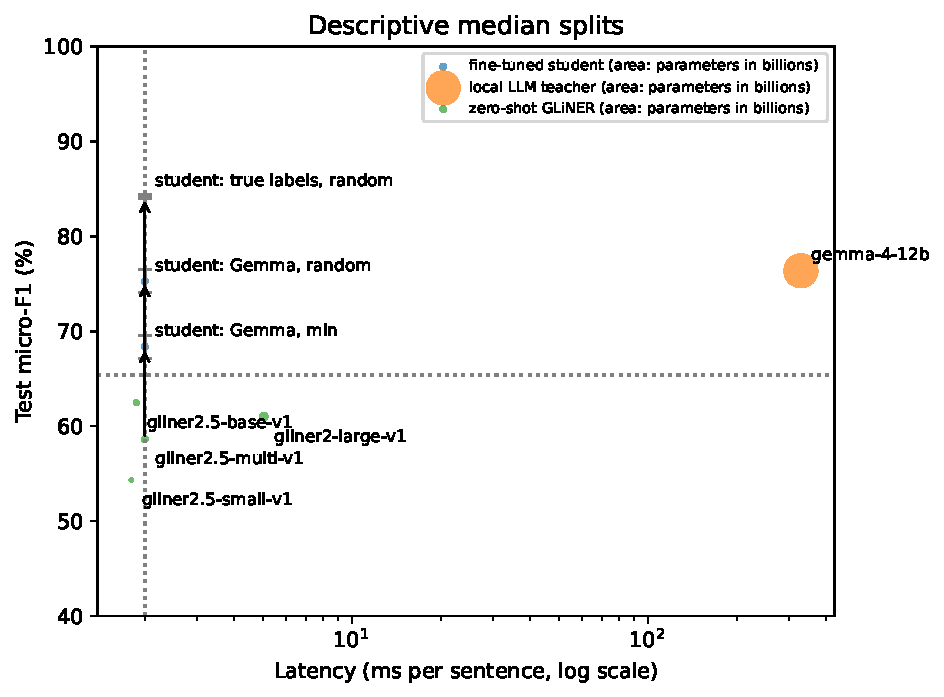
\includegraphics[width=\columnwidth]{figures/deployment-ner/quadrants.pdf}
\caption{NER, pooled over the three datasets: test micro-F1 against latency on one RTX 3090. Dotted lines are medians. Arrows lead from the zero-shot student to fine-tuned students (400 sentences). Error bars: seed SD.}
\label{fig:quadrant}
\end{figure}

\paragraph{Q7: cost and speed.} Figure~\ref{fig:quadrant} places students and teacher on one chart for NER, pooled over the three datasets. Gemma~4 12B labels at \res{DeployTeacherLatency} ms per sentence and reaches \res{DeployTeacher} F1. A student trained on 400 random Gemma-labelled sentences reaches \res{DeployStudentGemmaRandom} at \res{DeployStudentGemmaRandomLatency} ms, \res{DeploySpeedup} times faster; the estimated inference cost falls from \res{DeployTeacherCost} to \res{DeployStudentGemmaRandomCost} USD per million sentences. The same student trained on 400 ground-truth sentences reaches \res{DeployStudentTrueRandom}, and on 400 Gemma labels picked by min only \res{DeployStudentGemmaMin}; the untrained student scores \res{DeployZeroShot}. The Pareto front (Figure~\ref{fig:pareto}), learning curves (Figure~\ref{fig:learning}) and per-dataset cost curves, which add labelling and selection cost (Figure~\ref{fig:cost}), are in Appendix~\ref{sec:appendix}.

\subsection{Replicating the thesis experiments}
\label{sec:replication}

We reran the thesis experiments on all seven dataset cells with the protocol above: three seeds, a frozen pool, and dev for every choice.

\paragraph{Thesis selectors measure noise.} The thesis compared three sentence scores: mean confidence (avg), mean squared error from full confidence (MSE) and mean negative log-probability (MNLP). In all \res{ThesisSelectorCells} cells (dataset, label source, budget and seed) the three scores select exactly the same sentences (\res{ThesisSelectorIdenticalCells} of \res{ThesisSelectorCells}). Each score ranks a sentence with no prediction as least confident, and every pool holds more such sentences than the largest thesis budget: from \res{MITMovieNoPredictionCount} (\res{MITMovieNoPredictionShare}\%) on MIT Movie to \res{HallmarksNoPredictionCount} (\res{HallmarksNoPredictionShare}\%) on Hallmarks. The selected set is therefore a seeded random draw of empty sentences. For NER, min uses the same rule and selects the same set too (\res{ThesisSelectorNERMinIdenticalCells} of \res{ThesisSelectorNERCells} cells). Any score difference between avg, MSE and MNLP is training noise, which makes them a free repeatability test: with the same sentences and seeds, mean F1 differs by up to \res{HallmarksGroundTruthThesisSpread} points on Hallmarks, \res{CrossREGroundTruthThesisSpread} on CrossRE and \res{MassiveEnGemmaThesisSpread} on MASSIVE English, but only \res{BCfiveCDRGroundTruthThesisSpread} on BC5CDR with ground truth. The thesis ranking of these scores cannot be read as a ranking of methods.

\paragraph{Which weights to train.} The default student trains LoRA adapters on the encoder and the task heads. With 400 random ground-truth sentences (three seeds), adapters on the encoder alone score within one point of the default on every dataset (MIT Movie \res{MITMovieEncoderOnly} against \res{MITMovieGroundTruthRandom}, Hallmarks \res{HallmarksEncoderOnly} against \res{HallmarksGroundTruthRandom}). Training the heads alone loses heavily everywhere (CleanCoNLL \res{CleanCoNLLHeadsOnly} against \res{CleanCoNLLGroundTruthRandom}, MASSIVE English \res{MassiveEnHeadsOnly} against \res{MassiveEnGroundTruthRandom}, BC5CDR \res{BCfiveCDRHeadsOnly} against \res{BCfiveCDRGroundTruthRandom}) and collapses on Hallmarks (\res{HallmarksHeadsOnly}). The encoder carries the adaptation. Full fine-tuning of all weights on the whole ground-truth pool (one seed, learning rate not tuned) scores below LoRA on the whole pool for BC5CDR (\res{BCfiveCDRFullFinetune} against \res{BCfiveCDRGroundTruthWholePool}), CleanCoNLL (\res{CleanCoNLLFullFinetune} against \res{CleanCoNLLGroundTruthWholePool}), MIT Movie (\res{MITMovieFullFinetune} against \res{MITMovieGroundTruthWholePool}) and MASSIVE English (\res{MassiveEnFullFinetune} against \res{MassiveEnGroundTruthWholePool}). It is higher only on Hallmarks (\res{HallmarksFullFinetune} against \res{HallmarksGroundTruthWholePool}), where the LoRA run stopped early (Limitations). LoRA is enough for this student.

\paragraph{Thresholds and budgets.} The thesis tuned the decision threshold on test data. On dev, the threshold matters for the zero-shot student and hardly at all after training: dev F1 moves by up to \res{HallmarksZeroShotSpread} points across thresholds 0.3 to 0.7 for the zero-shot student on Hallmarks (\res{MassiveEnZeroShotSpread} on MASSIVE English), against at most \res{CrossRETrainedSpread} for a trained student on any dataset. The learning curves over budgets from 50 to 1{,}000 sentences are in Figure~\ref{fig:learning}.

\section{What the thesis did, and what this study fixes}
\label{sec:thesis}

The thesis ran sixteen experiments on MIT Movie: zero-shot and fully fine-tuned GLiNER, an Optuna search and a LoRA layer study, confidence brackets and a threshold sweep, four selection scores over fourteen budgets, a hard-example comparison of GLiNER and Gemma~3, students on LLM versus ground-truth labels, a mixing grid of ground truth and LLM labels, four teachers, synthetic data, a prompt validator and a cost study. It found, without stating it openly, that Gemma~3's F1 drops from 69.4 on the full test set to 56.9 on the 100 training sentences where GLiNER was least confident; this study turns that observation into question Q2.

The thesis protocol had problems that this study fixes: the MIT Movie dev file was a copy of the test file, so Optuna, early stopping and threshold choice used test data; the pool filter removed sentences with no ground-truth entity; the saved adapter was the last checkpoint rather than the best; the Optuna pruner never received intermediate scores; and no result was repeated with a second seed. Rerun under the fixed protocol on all datasets (Section~\ref{sec:replication}), two thesis conclusions do not hold: its three selection scores pick the same sentences, so their ranking was noise, and its mixing result holds on MIT Movie only.

\section{Limitations}

Our results cover one round of selection, one student family and English plus French data. CrossRE uses given entity mentions, so its results do not cover end-to-end relation extraction. The hyphen-free tokenisation of the datasets hides a GLiNER2 word-splitting issue that matters for raw biomedical text. We cannot rule out that our models saw the evaluation data. No model owner states that our six datasets were in training, and none states that they were removed. The GLiNER2 family reports zero-shot results on CrossNER, whose sentences and splits CrossRE reuses, so CrossRE test sentences were part of the student developers' entity evaluation; whether checkpoints were chosen on them is unknown. The student's training text includes news and PubMed, so the text (not the labels) of CleanCoNLL, BC5CDR and Hallmarks may overlap. CoNLL-2003 is a known contamination case for earlier LLMs, and public instruction collections contain CoNLL and BC5CDR tasks; our teachers do not document whether such data was used. MASSIVE postdates the student encoder's pre-training text. The full audit is in Appendix~\ref{sec:audit}. Training is not exactly repeatable on our GPU. NER runs on ground truth repeat almost to the digit (identical selections differ by at most \res{MITMovieGroundTruthThesisSpread} points), but relation, classification and slot runs, and NER runs on Gemma labels, can differ by up to \res{HallmarksGroundTruthThesisSpread} points on the same sentences and seed (Section~\ref{sec:replication}). We therefore report the seed SD of every cell and of every contrast. Costs are estimates: GPU time at one rental price on one date, and ground-truth labels at a simulated crowd rate of 0.50 USD per sentence taken from a span-annotation study \citep{kasner2026spanannotators}. The planned API teachers (Qwen and gpt-oss on Cerebras) were not run, so every teacher in this study is a local Gemma model, and the smaller E4B teacher labelled only the ladder samples and two training cells.

Three further points qualify single cells. The whole-pool Hallmarks run stopped early on a dev plateau, so it understates what the full pool can give; sentence-level Hallmarks is also much harder than the abstract-level task on which published scores are reported. Six CrossRE runs stopped with a non-finite gradient and one MASSIVE run made no optimiser step; all ran again with the same configuration and seed and finished normally. Runs killed by a GPU fault or out of memory were restarted in a new process with the same configuration and seed. The GLiNER2 trainer silently skips a batch that runs out of GPU memory; a check of epoch against step count in every training log found five runs with skipped batches. We made out of memory stop the run, and those five runs were repeated in full. Finally, fine-tuned students were not timed separately: they reuse the zero-shot timing of their base model, on the unmeasured assumption that a LoRA adapter adds little inference time.

\section*{Ethics and broader impact}

All datasets are public and used for research as intended by their licences. We release teacher labels as sentence ids and character offsets, never text whose licence forbids it. No human annotators were involved. The GPU time of every run is in the released run logs.

\section*{Use of AI assistants}

The first version of the code was written by an AI coding assistant (OpenAI Codex) and reviewed by a second assistant (Anthropic Claude), which wrote the later code, fixes and analysis, helped plan experiments and drafted text. The author checked the design, the results and every citation, and takes responsibility for the content.

\bibliography{references,references_extra}

\appendix

\section{Additional figures}
\label{sec:appendix}

\newcommand{\panel}[1]{\includegraphics[width=0.32\textwidth]{figures/#1.pdf}}

\begin{figure}[h]
\centering
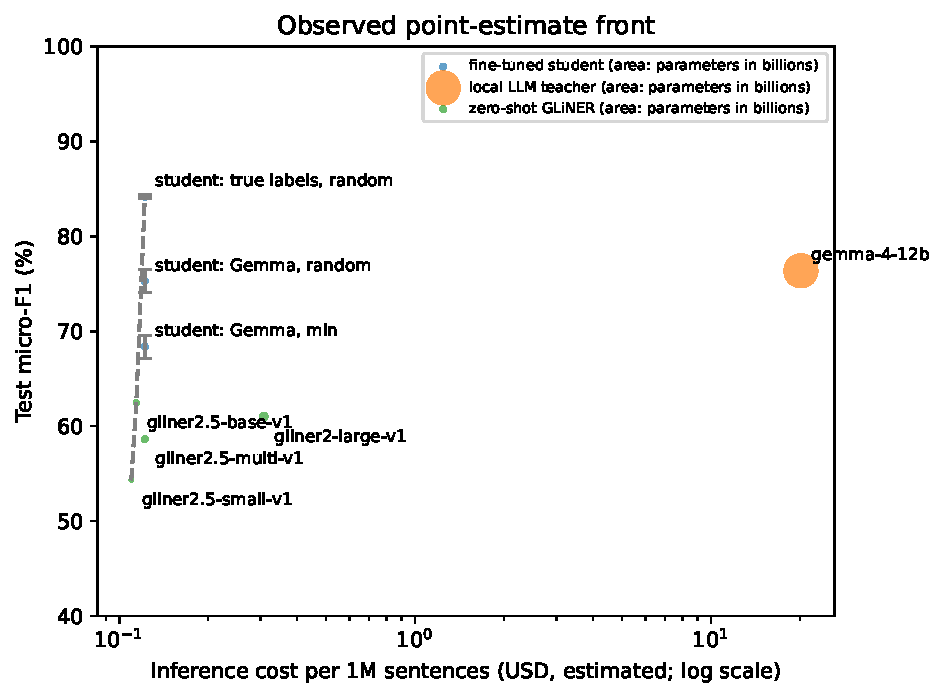
\includegraphics[width=\columnwidth]{figures/deployment-ner/pareto.pdf}
\caption{NER, pooled over three datasets: test micro-F1 against estimated inference cost per million sentences (GPU time at one rental price). The dashed line joins the observed points that no other point beats on both axes.}
\label{fig:pareto}
\end{figure}

\begin{figure*}[t]
\centering
\panel{learning-cleanconll-en-US}\hfill\panel{learning-bc5cdr-en-US}\hfill\panel{learning-mit_movie-en-US}\\
\panel{learning-crossre-en-US}\hfill\panel{learning-hallmarks-en-US}\hfill\panel{learning-massive-en-US}\\
\panel{learning-massive-fr-FR}
\caption{Test micro-F1 against the number of labelled sentences. Solid lines: ground truth; dashed lines: Gemma~4 12B labels. Grey lines: whole pool; dotted line: zero-shot student. Error bars: seed SD.}
\label{fig:learning}
\end{figure*}

\begin{figure*}[t]
\centering
\panel{cost-cleanconll-en-US}\hfill\panel{cost-bc5cdr-en-US}\hfill\panel{cost-mit_movie-en-US}\\
\panel{cost-crossre-en-US}\hfill\panel{cost-hallmarks-en-US}\hfill\panel{cost-massive-en-US}\\
\panel{cost-massive-fr-FR}
\caption{Test micro-F1 against estimated labelling cost: ground truth at a simulated 0.50 USD per sentence, Gemma labels at free-GPU time, plus pool scoring for min and diversity.}
\label{fig:cost}
\end{figure*}

\section{Data overlap audit}
\label{sec:audit}

We checked papers, model cards and technical reports (September 2026) for each pair of evaluation dataset and model. We ran no probe, so nothing in this section is measured. Table~\ref{tab:audit} gives the result. No model owner states that any of our datasets was in training, and none states that it was removed.

\begin{table}[h]
\centering
\small
\begin{tabular}{lccc}
\toprule
Dataset & Student & Encoder & Teachers \\
\midrule
CleanCoNLL & U & U & P, high \\
BC5CDR & U & P & P \\
MIT Movie & U & U & P, low \\
CrossRE & E & P & P, high \\
Hallmarks & U & P & P \\
MASSIVE & U & N & P \\
\bottomrule
\end{tabular}
\caption{Possible overlap of evaluation data with model training data. E: evaluated on by the model owner; P: a named path exists but no source confirms it; N: not possible by date; U: unknown. Student: GLiNER2.5-multi; encoder: mDeBERTa-v3 (CC-100); teachers: Gemma~4 E4B and 12B.}
\label{tab:audit}
\end{table}

\paragraph{Student.} The GLiNER2.5 release states that its training data was generated by an agent rather than assembled from existing datasets; it names no teacher, corpus or size and makes no decontamination statement \citep{gliner25multi}. It reports zero-shot results on five CrossNER domains. CrossRE annotates relations on the CrossNER sentences with the same splits \citep{crossre2022}, so the student's developers have scored entities on our CrossRE test sentences; whether they chose checkpoints on those scores is unknown. GLiNER2 trains on news, Wikipedia and PubMed text labelled by GPT-4o \citep{gliner2_2025}, so the text, not the labels, of BC5CDR, Hallmarks and CrossRE may overlap with the zero-shot ladder models.

\paragraph{Encoder.} mDeBERTa-v3 is pre-trained on CC-100, built from 2018 Common Crawl snapshots. MASSIVE (2022) and its source SLURP (2020) cannot be in it. Wikipedia and PubMed pages can be, so CrossRE, BC5CDR and Hallmarks text may be familiar to the encoder; a masked encoder sees text without our labels.

\paragraph{Teachers.} Every dataset was public before the Gemma~4 data cutoff (January 2025). The Gemma~4 report states that benchmarks were decontaminated but does not list them. CoNLL-2003 is a documented contamination case for ChatGPT, which reproduces its test sentences with labels. Public instruction collections contain CoNLL and BC5CDR tasks; no teacher owner says whether it used them. We therefore treat CleanCoNLL and the news domain of CrossRE, which is CoNLL-2003 text, as likely seen by the teachers.

\paragraph{Effect on our claims.} Exposure raises absolute teacher and student scores. Our main claims compare selection arms, and teachers, on the same sentences. Exposure that is equal across arms does not bias these paired contrasts, but it can narrow the measured gap between teacher labels and ground truth. MASSIVE English and French are translations of the same utterances, so the two locales are not independent evidence.

\end{document}
